\documentclass[a4paper,11pt]{scrartcl}

\usepackage[english]{babel}

\usepackage[utf8]{inputenc} 
\usepackage[T1]{fontenc}
\usepackage{lmodern, mathpazo}
%\usepackage{helvet}
\usepackage{csquotes}
%\usepackage{musixtex}

\usepackage{amsmath, amsfonts, mathtools, amssymb}

\usepackage{etex}

\usepackage{tikz}
\usepackage{tikz-network}
\usepackage[hidelinks]{hyperref}
\usepackage[english, nameinlink, capitalise]{cleveref}
\usepackage[
    backend=biber,
    bibencoding=utf8,
    sorting=none,
    url=false,
    doi=false
]{biblatex}
\addbibresource{uni23.bib}

\usepackage{listings}

\usepackage{siunitx}
\DeclareSIUnit\nat{nat}
%\usepackage[onehalfspacing]{setspace}
\usepackage{graphicx}                   % Bilder
%\usepackage{floatflt}               % flt 
\usepackage{float}
\usepackage{physics}

\usepackage{caption}

\usepackage{amssymb}
\usepackage{amsmath}
%\usepackage{pgfplots}
\crefname{ineq}{ineq.}{inequalities}
\creflabelformat{ineq}{#2{\upshape(#1)}#3}
\author{}
\RequirePackage{etex}
\title{Review of results}
%\date{\today}

\begin{document}
\maketitle
\section{Introduction}
In \citeyear{BA_Pendry_1983}, \citeauthor{BA_Pendry_1983} derived a bound on the flow of information, which reads
\begin{align}\label[ineq]{eq:pendry}
    \dot{I}^2 \leq \frac{\pi}{3\hbar\ln^22}\dot{E}.
\end{align}
This result is derived using classical statistical mechanics \cite{BA_Pendry_1983}. However, this classical framework
neglects the effects of genuine quantum mechanical phenomena, such as quantum correlations.
We show that this inequality is violated in a model system with quantum correlations, and provide a bound on information flow,
which corrects for contributions from correlations.
\section{The model}
Consider a chain of qubits in the Heisenberg-$XY$ model. Restricting their interaction to their nearest neighbors allows
us to draw a comparison to Pendry's original derivation with fermions using Jordan-Wigner transform, mapping a chain of
spin-$1/2$ qubits to a chain of spinless fermions. The information flow is then the time derivative of 

In particular, we have the Hamiltonian of this system as
\begin{align}\label{eq:hamiltonian-perfect-transfer}
    H &= -\sum\limits_i \sigma^z_i + \sum\limits_j \frac{J_j}{2} (\sigma^x_j\sigma^x_{j+1}+\sigma^y_j\sigma^y_{j+1})\\
    \shortintertext{with}
    J_k &= \frac{\lambda}{2}\sqrt{j\cdot(N-j)}.\nonumber
\end{align}
This ensures a predictable periodic behaviour of the chain. This can be made apparent by considering the local
magnetization $\expval{\sigma^z_i}$ of the qubits. \Cref{fig:no-corr} shows the time evolution of the quibts'
magnetization.\footnote{We choose $\lambda$ to be $1$. It was shown in \cite{BA_Christandl_2004} that at
time $t=\pi/\lambda$, perfect state transfer is achieved}
\begin{figure}[H]
    \centering
    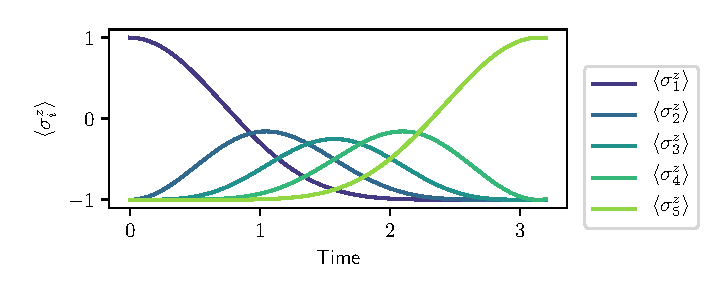
\includegraphics{expval_z.pdf}
    \caption{Time evolution of the individual magnetizations $\expval{\sigma^z_i}$ for the system with
    Hamiltonian defined as in \cref{eq:hamiltonian-perfect-transfer}.
    Qubit $i=1$ is prepared in the excited state at time $t=0$.
    Qubits $i>1$ are prepared in the ground state at time $t=0$.}
    \label{fig:no-corr}
\end{figure}
This perfect transfer works for an arbitrary initial state and size of the system. Consider \cref{fig:no-corr-thermal},
where we scaled up the system to include $N=6$ qubits and have the initial state of qubit $1$ and $2$ as a thermal state.
\begin{figure}
    \centering
    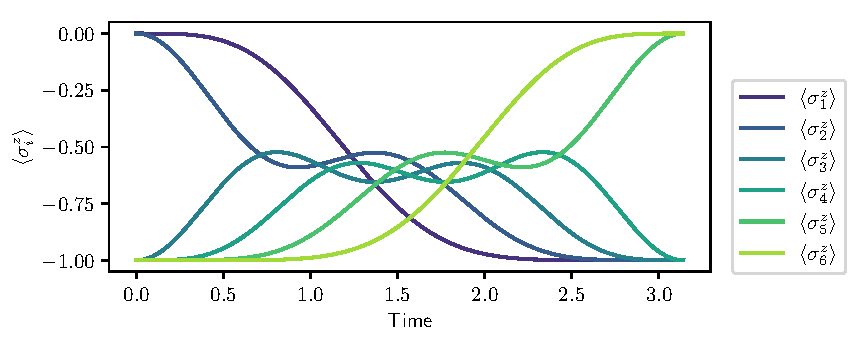
\includegraphics{thermal-state-expval-z-no-corr.pdf}
    \caption{Time Evolution of the individual magnetizations of the qubits
    $\expval{\sigma^z_i}$, where the interaction is governed by \cref{eq:hamiltonian-perfect-transfer}.
    Qubits $i=1$ and $i=2$ are initially prepared in a thermal state $\rho_{1,2} = \exp(-\beta_{1,2}\sigma^z_{1,2})/Z$
    and qubits $i\neq1,2$ are prepared in the ground state.}
    \label{fig:no-corr-thermal}
\end{figure}
We can verify if \cref{eq:pendry} holds. \Cref{fig:pendry-thermal} shows the information and energy flow over time. Here, information flow
%(in units of $\si{\nat\per\second}$)
is given by
\begin{align}\label{eq:i-dot-sq}
    \dot{I} = -\partial_t \Tr[\rho\ln\rho].
\end{align}
\begin{figure}[H]
    \centering
    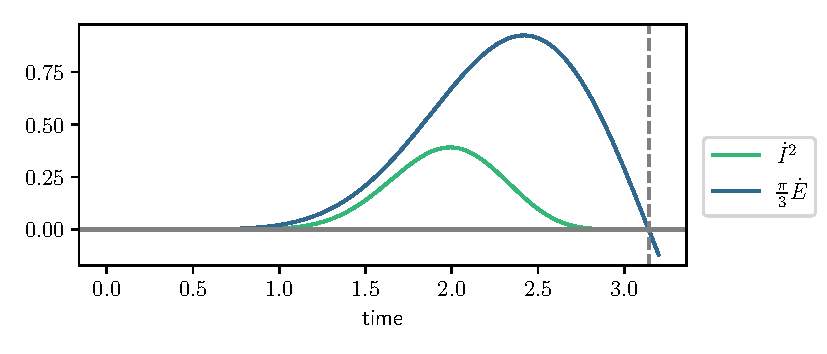
\includegraphics{pendry_propagate_thermal_state_energy_without_ln2_new.pdf}
    \caption{Information and energy flow of the last qubit in the chain. Here, the chain propagates a thermal state from one end to the other.}
    \label{fig:pendry-thermal}
\end{figure}
\section{Quantum correlations}
In a work by \citeauthor{BA_kaonan_correlations}, it was shown that certain quantum correlations
\emph{invert} the flow of energy \cite{BA_kaonan_correlations}. Heat flows, initially, not from hot to cold, but
from cold to hot. The two-qubit state is then described by a product state with an added correlation term of the form
\begin{align}\label{eq:kaonans-corr}
    \chi = -i\alpha(\sigma^+_k \sigma^-_{k+1} - \sigma^-_k \sigma^+_{k+1}),
\end{align}
with 
\begin{align}\label{eq:alpha-max}
    \abs{\alpha_\text{max}} = \frac{1}{4\cosh\beta_1\cosh\beta_2}.
\end{align}
\Cref{fig:corr} shows the chain with initial correlations at positions 1 and 2 of the chain.
\begin{figure}[H]
    \centering
    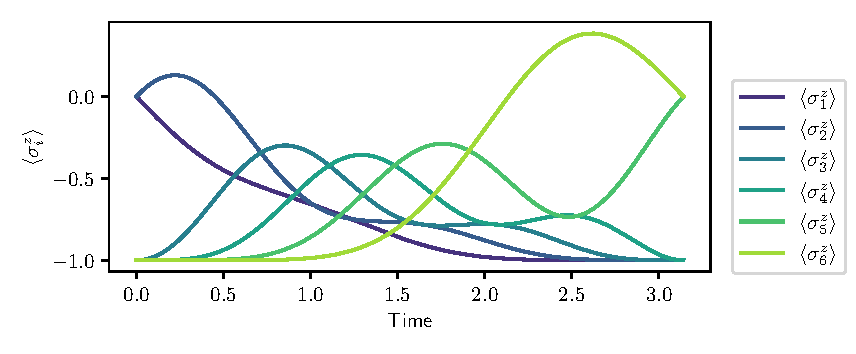
\includegraphics{thermal-state-expval-z-corr.pdf}
    \caption{Time Evolution of the individual magnetizations of the qubits
    $\expval{\sigma^z_i}$, where the interaction is governed by \cref{eq:hamiltonian-perfect-transfer}.
    Qubits $i=1$ and $i=2$ are prepared in an initially correlated state $\rho_{12} = \rho_1 \otimes \rho_2 + \chi$
    and qubits $i\neq1,2$ are prepared in the ground state.
    Locally, Qubit $1$ and $2$ are in a thermal state each, with identical inverse temperature $\beta = 1/300$.}
    \label{fig:corr}
\end{figure}
This dynamics has implications on \cref{eq:pendry}. \Cref{fig:corr12_pendry} shows the analogous plot to \cref{fig:pendry-thermal}.
\begin{figure}[H]
    \centering
    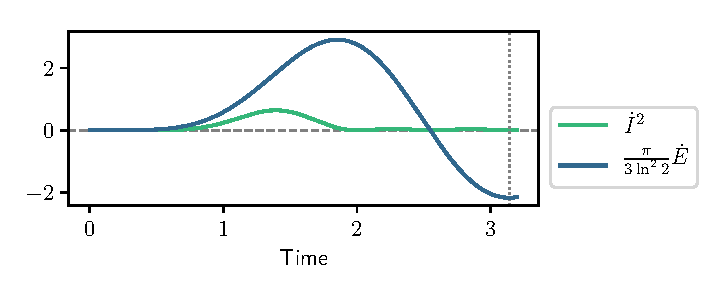
\includegraphics{12_penry_grey_lines_first_thermal.pdf}
    \caption{Energy flow  and information flow of qubit $N$ for 
    initially correlated qubits $1$ and $2$.
    The dotted vertical line indicates $t=\pi$, which is the time of state inversion, i.e. where the dynamics reverse,
    dictated by the interaction.}
    \label{fig:corr12_pendry}
\end{figure}
This shows that this type of initial state leads to a reversal of heat flow and, as a consequence, to a violation of \cref{eq:pendry}.
\subsection{Bound on information flow}
Seeing as we are able to violate \cref{eq:pendry}, we are now interested in a more general bound, which also holds for systems
with quantum correlations.

As preliminaries, we separate correlated and uncorrelated energy flow,
\begin{align}
    \dot{E} = \dot{E}_0^t + \dot{E}_\chi^t,
\end{align}
with subscript $\chi$ denoting contributions from correlations,
and rewritie quantum relative entropy as
\begin{align}
    \mathcal{S}(\rho^t\mid\mid\rho^0_\text{th}) = - \Delta S + \beta \Delta E.
\end{align}
Taking time derivative and isolating $\dot{S}$,
\begin{align}
    \dot{S}_0 &= \beta \dot{E}_0^t- \dot{\mathcal{S}}_0(\rho^t_N \mid \mid \rho^0_N)\label{eq:dotVN_no_chi}\\
    \dot{S} &= \beta \left(\dot{E}_0^t + \dot{E}_\chi^t\right)
    - \dot{\mathcal{S}}_\chi(\rho^t_N \mid \mid \rho^0_N)\label{eq:dotVN_with_chi}
\end{align}
After subtracting eq. \eqref{eq:dotVN_no_chi} from eq. \eqref{eq:dotVN_with_chi} one has
\begin{align}
    \dot{S} - \dot{S}_0 = \beta \dot{E}_\chi^t - \Delta_\chi \dot{\mathcal{S}}(\rho^t_N \mid \mid \rho^0_N)
\end{align}
Isolating $\dot{S}$ again, then squaring the result gives the exact result of
\begin{align}
    \dot{S}^2 = \left(\dot{S}_0 + \beta \dot{E}_\chi - \Delta_\chi \dot{\mathcal{S}}\left(\rho^t_N \mid \mid \rho^0_N\right)\right)^2
\end{align}
Inserting \cref{eq:pendry} into above expression we obtain
\begin{equation}\label[ineq]{ineq:newbound}
    \dot{S}^2 \leq \frac{\pi}{3\ln^22} \dot{E}^t_0 + 2\dot{S}_0\left(\beta \dot{E}_\chi - \Delta \dot{\mathcal{S}}\left(\rho^t_N \mid \mid \rho^0_N\right)\right) + \left(\beta \dot{E}_\chi - \Delta \dot{\mathcal{S}}\left(\rho^t_N \mid \mid \rho^0_N\right)\right)^2
\end{equation}

\Cref{fig:newbound_corr12_same_beta_with_old} shows the comparisons of the previous and the corrected bound.
\begin{figure}[H]
    \centering
    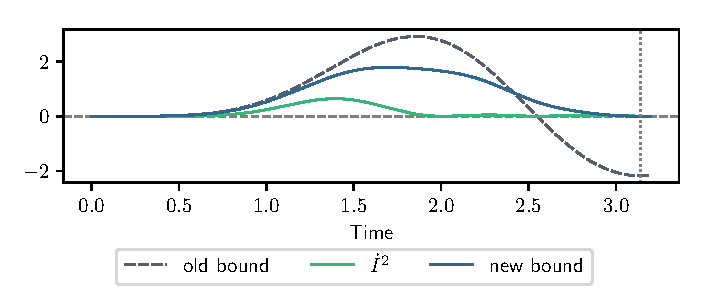
\includegraphics{corr12_beta1=beta2_new_with_old_bound.pdf}
    \caption{Bound according to \cref{ineq:newbound}. "Old bound" given by \cref{eq:pendry}.
    In the case shown, qubit $1$ and qubit $2$ are correlated with equal temperatures $\beta = 1/300$.}
    \label{fig:newbound_corr12_same_beta_with_old} 
\end{figure}
\subsection{Dependence of the dynamics on quantum discord}
The quantum-ness of the correlations can be quantified through \emph{geometric discord}.
We investigate the dependence of certain quantities on discord by varying $\alpha$ in \cref{eq:kaonans-corr}.
\Cref{fig:inf-as-func-of-disc} shows the reduced maximum information flow. 
\begin{figure}[H]
    \centering
    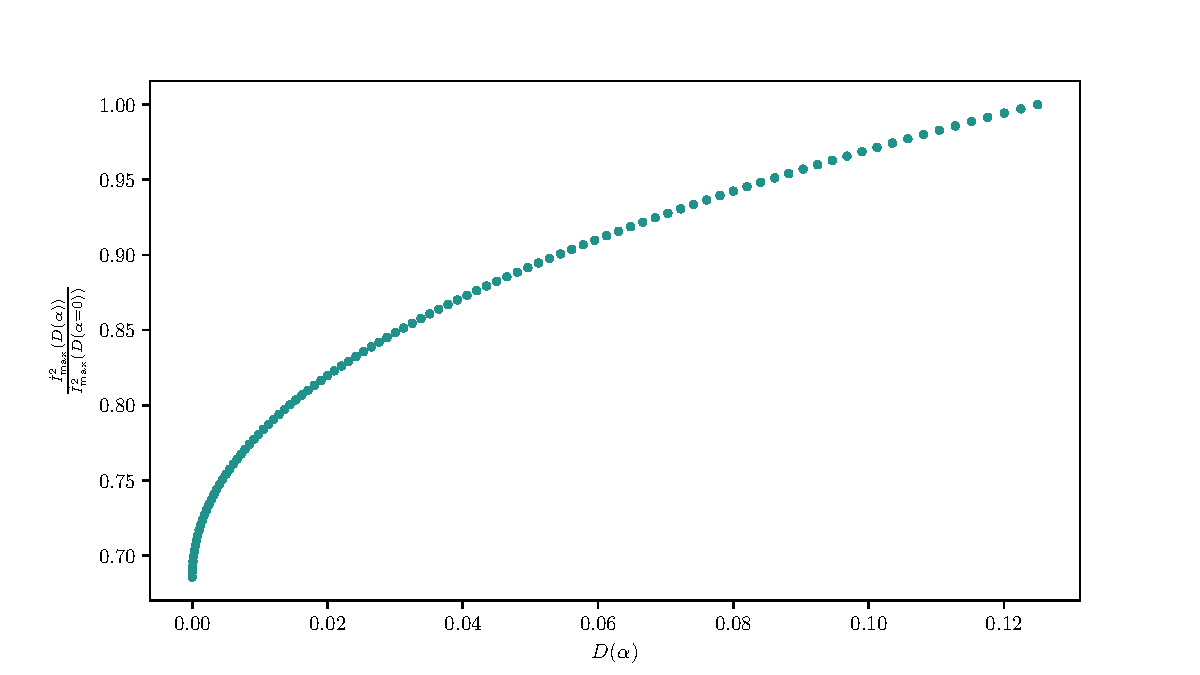
\includegraphics[width=\textwidth]{i_dot_sq_max_reduced_of_discord.pdf}
    \caption{Reduced maximum information flow as a function of discord. The values for information flow are divided
    by the maximum, $\dot{I}^2_\mathrm{max}[D(\alpha=\alpha_\mathrm{max})]$, such that the range is from $0$ to $1$.}
    \label{fig:inf-as-func-of-disc}
\end{figure}
We also investigate the fidelity of the first and last qubits, either as pairs of or as separate qubits.
\Cref{fig:gridplot-fid-of-disc} shows the fidelity as a function of time for two different values of the geometric discord.
\begin{figure}[H]
    \centering
    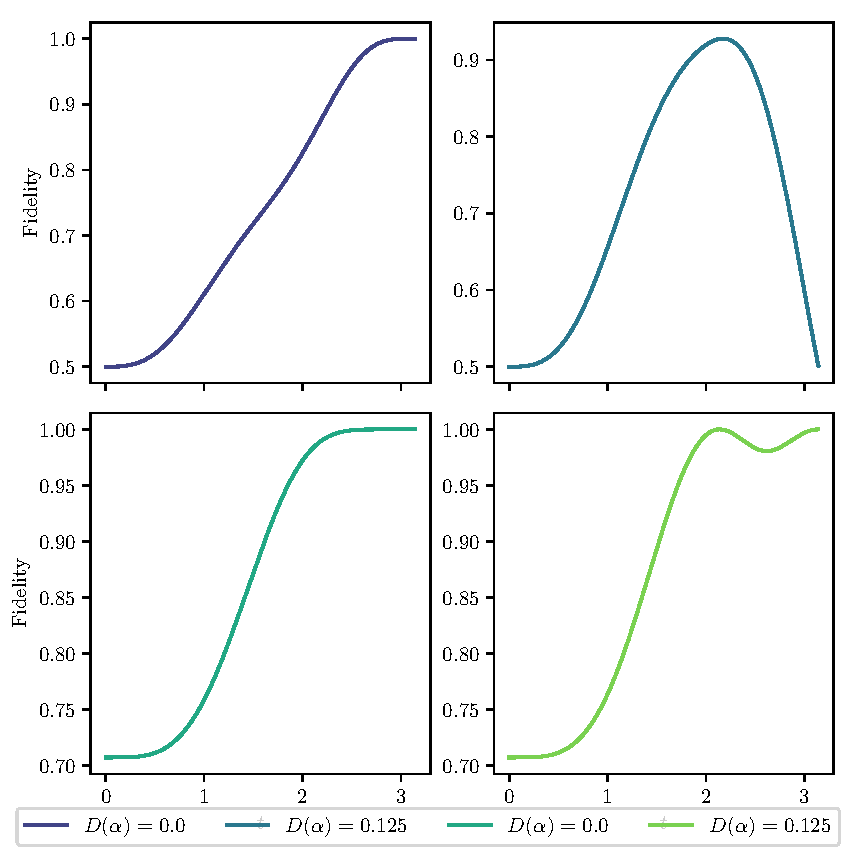
\includegraphics{max_und_min_discord_fidelities.pdf}
    \caption{Fidelity of the last qubit with the initial state of the first qubit
    as a function of time for minimal (maximal) discord (top/bottom left).
    On the right: Fidelity of the last two qubits with the initial state of the first two
    as a function of time for minimal (maximal) discord}
    \label{fig:gridplot-fid-of-disc}
\end{figure}
\Cref{fig:gridplot-fid-of-disc} shows that when considering the single qubits, we have a state transfer, which
occurs at an earlier point than $t=\pi$. This \emph{arrival time} can also be plotted as a function of geometric discord.
\Cref{fig:arr-time} shows this relation.
\begin{figure}[H]
    \centering
    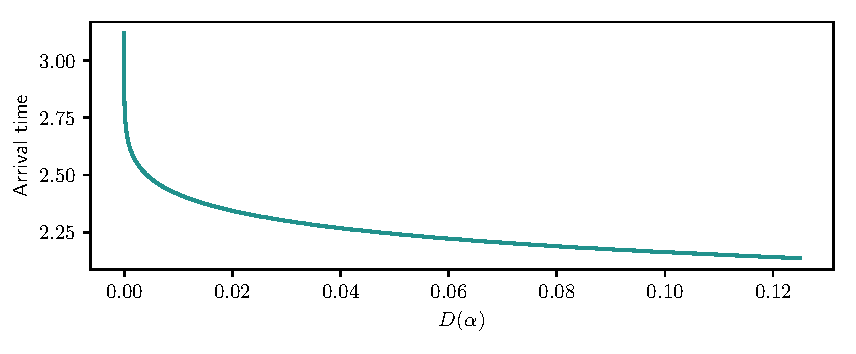
\includegraphics{arr_time_over_discord.pdf}
    \caption{Arrival time (first local maximum in fidelity) as a function of geometric discord.}
    \label{fig:arr-time}
\end{figure}
%\begin{figure}
%    \centering
%    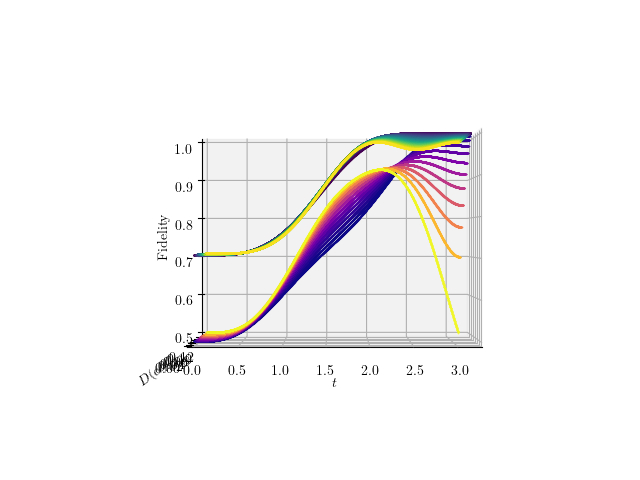
\includegraphics[width=\textwidth]{twoqubit_and_local_fidelity_of_t_against_discord.png}
%    \caption{local fidelity and fidelity of two qubits as a function of time and discord}
%    \label{fig:3dplot-fid-of-disc}
%\end{figure}

%\begin{displayquote}
%Since energy is conserved the flow into this segment equals the
%flow out and therefore energy flow is conserved as is the particle flow. However,
%the entropy flow is not conserved but can only increase monotonically until thermal
%equilibrium is established.
%\end{displayquote}
\printbibliography
\end{document}
